
\chapter{Calculation of Hydrodynamic Stresses on Stems of an Emergent Vegetation
Layer using a Unit-Cell Meshing Method: OpenFOAM Simulations}

\section{Introduction}

Natural vegetation layers located in water bodies play an important
role in ecosystems by providing shelter for aquatic life and reducing
land erosion. For example, coastal vegetation layers such as coral
reefs can be located in tropical oceans near the equator such as those
we have surrounding the Hawaiian Islands, yet they have proven to
be one on the most sensitively vulnerable groups threatened by global
warming \citep{silbiger_environmental_2017}. Although vital for biodiversity
and shoreline protection, countless physical, chemical and biological
stressors, as complexly coupled, make it difficult for researchers
to predict consequential responses of vegetation due to future environmental
changes \citep{zhu_biomechanical_2019,folkard_biophysical_2019}.
Sea level rise, for example, has increasingly been found to influence
coastal degradation within the Hawaiian Islands, contributing to nearly
52--78\% of the state\textquoteright s beaches experiencing increased
rates of erosion \citep{romine_are_2013}. Globally, since the mid-2010s,
pilot programs with the intention of reducing vegetation loss, in
developing rural places such as the Caribbean Islands, have been initiated
for locally based communities to assess coastal vegetation reduction
and implement restoration efforts \citep{reguero_coral_2018}. However,
efficient vegetation structures for the civil and environmental engineering
practice to preserve the natural environment effectively, have not
yet been established. 

\section{Simulation Setup}

\subsection{Mesh Generation}

\subsubsection{Meshing script}

Fig. \ref{fig:blockMesh} shows ... 

\subsubsection{Vegetated (stem-occupied) cell}

Fig. \ref{fig:emptyStem} shows the mesh grids of void spaces in the
presence of a vertical, cylindrical stem embedded at the bed. The
central hole indicates the internal volume of the stem. The unit-cell
has seven boundaries, which include top, bottom, left, right, front,
and back. The stem was assumed to have a rigid interior and smooth
surfaces on which fluid velocity is assumed to be zero. A closer look
of Fig. \ref{fig:emptyStem}(a) indicates the mesh structure in the
unit-cell has a symmetry about the two diagonal lines and $x$- and
$y$-axes. In this case, a unidirectional flow far from the stem is
calculated implicitly using a rectangle-like grid and a detouring
flow around the stem is obtained using the polar grid.

\subsection{Shear stress}

Shear stress, in the engineering sector is one of the universally
used properties to describe sediment and debris transport through
an open channel\citep{petit_dimensionless_2015}. The term ``shear''
is defined as the force acting tangential to another object\textquoteright s
cross-sectional surface. A familiar analogy would be the river or
stream bed flow above the bed surface. Domestic agencies such as the
Vermont Agency of Natural Resources publish articles about construction
projects near or around river banks affecting shear stress as they
dictate the health of nearby ecosystems \citep{natural_resources_sediment_2004}.

In her review paper published in 2012, Heidi Nepf presented an approach
to predict bed stress for open-channel flow by defining it equal the
the spatial average of the viscous stress at the bed. This relationship
is also described as follows:

\begin{equation}
\tau_{bed}=\rho u_{*}^{2}=\left\langle \mu\frac{\partial\bar{u}}{\partial z}\mid_{z=0}\right\rangle \text{}\label{eq:}
\end{equation}
For this approach, $\frac{\partial\bar{u}}{\partial z}$ is the velocity
gradient normal to the surface above the vegetation bed surface \citep{nepf_hydrodynamics_2012}.

\section{Concluding Remarks}

\begin{onehalfspace}
In this chapter, we ...

Given our research at this point, we indicate  .... 
\end{onehalfspace}

\newpage\null
\vfill
\begin{table}[H]
\centering{}%
\begin{tabular}{|c|c|c|c|}
\hline 
Variables & Inlet & Outlet \& Top & Side \& Bottom Walls\tabularnewline
\hline 
\hline 
$p-\rho gh$ & Fixed-Flux-Pressure & Total-Pressure (0) & Fixed-Flux-Pressure\tabularnewline
\hline 
$U$ & Variable-Height-Inlet & Pressure-Inlet-Outlet-Velocity & No-Slip (U=0)\tabularnewline
\hline 
$\alpha$ & Inlet-Outlet (1) & Inlet-Outlet (0) & Zero-Gradient ($\nabla\text{\ensuremath{\alpha}}=0)$\tabularnewline
\hline 
\end{tabular}\caption{\label{tbl:coarseboundaryCond}Boundary condition parameters for the
coarse, moderate, and fine mesh.}
\end{table}

\vfill\newpage\null
\vfill
\begin{table}[H]
\centering{}%
\begin{tabular}{|c|c|c|}
\hline 
Mesh Fineness & Number of Internal Points & Approximate Run Time\tabularnewline
\hline 
\hline 
Coarse & 29,484 & 0 hr 20 min\tabularnewline
\hline 
Moderate & 69,888 & 1 hr 00 min\tabularnewline
\hline 
Fine & 136,500 & 5 hr 30 min\tabularnewline
\hline 
\end{tabular}\caption{\label{tbl:runtime}Simulation run times for the coarse, moderate,
and fine mesh.}
\end{table}

\vfill\newpage %\null
%\vfill
\begin{figure}[H]
\begin{centering}
(a)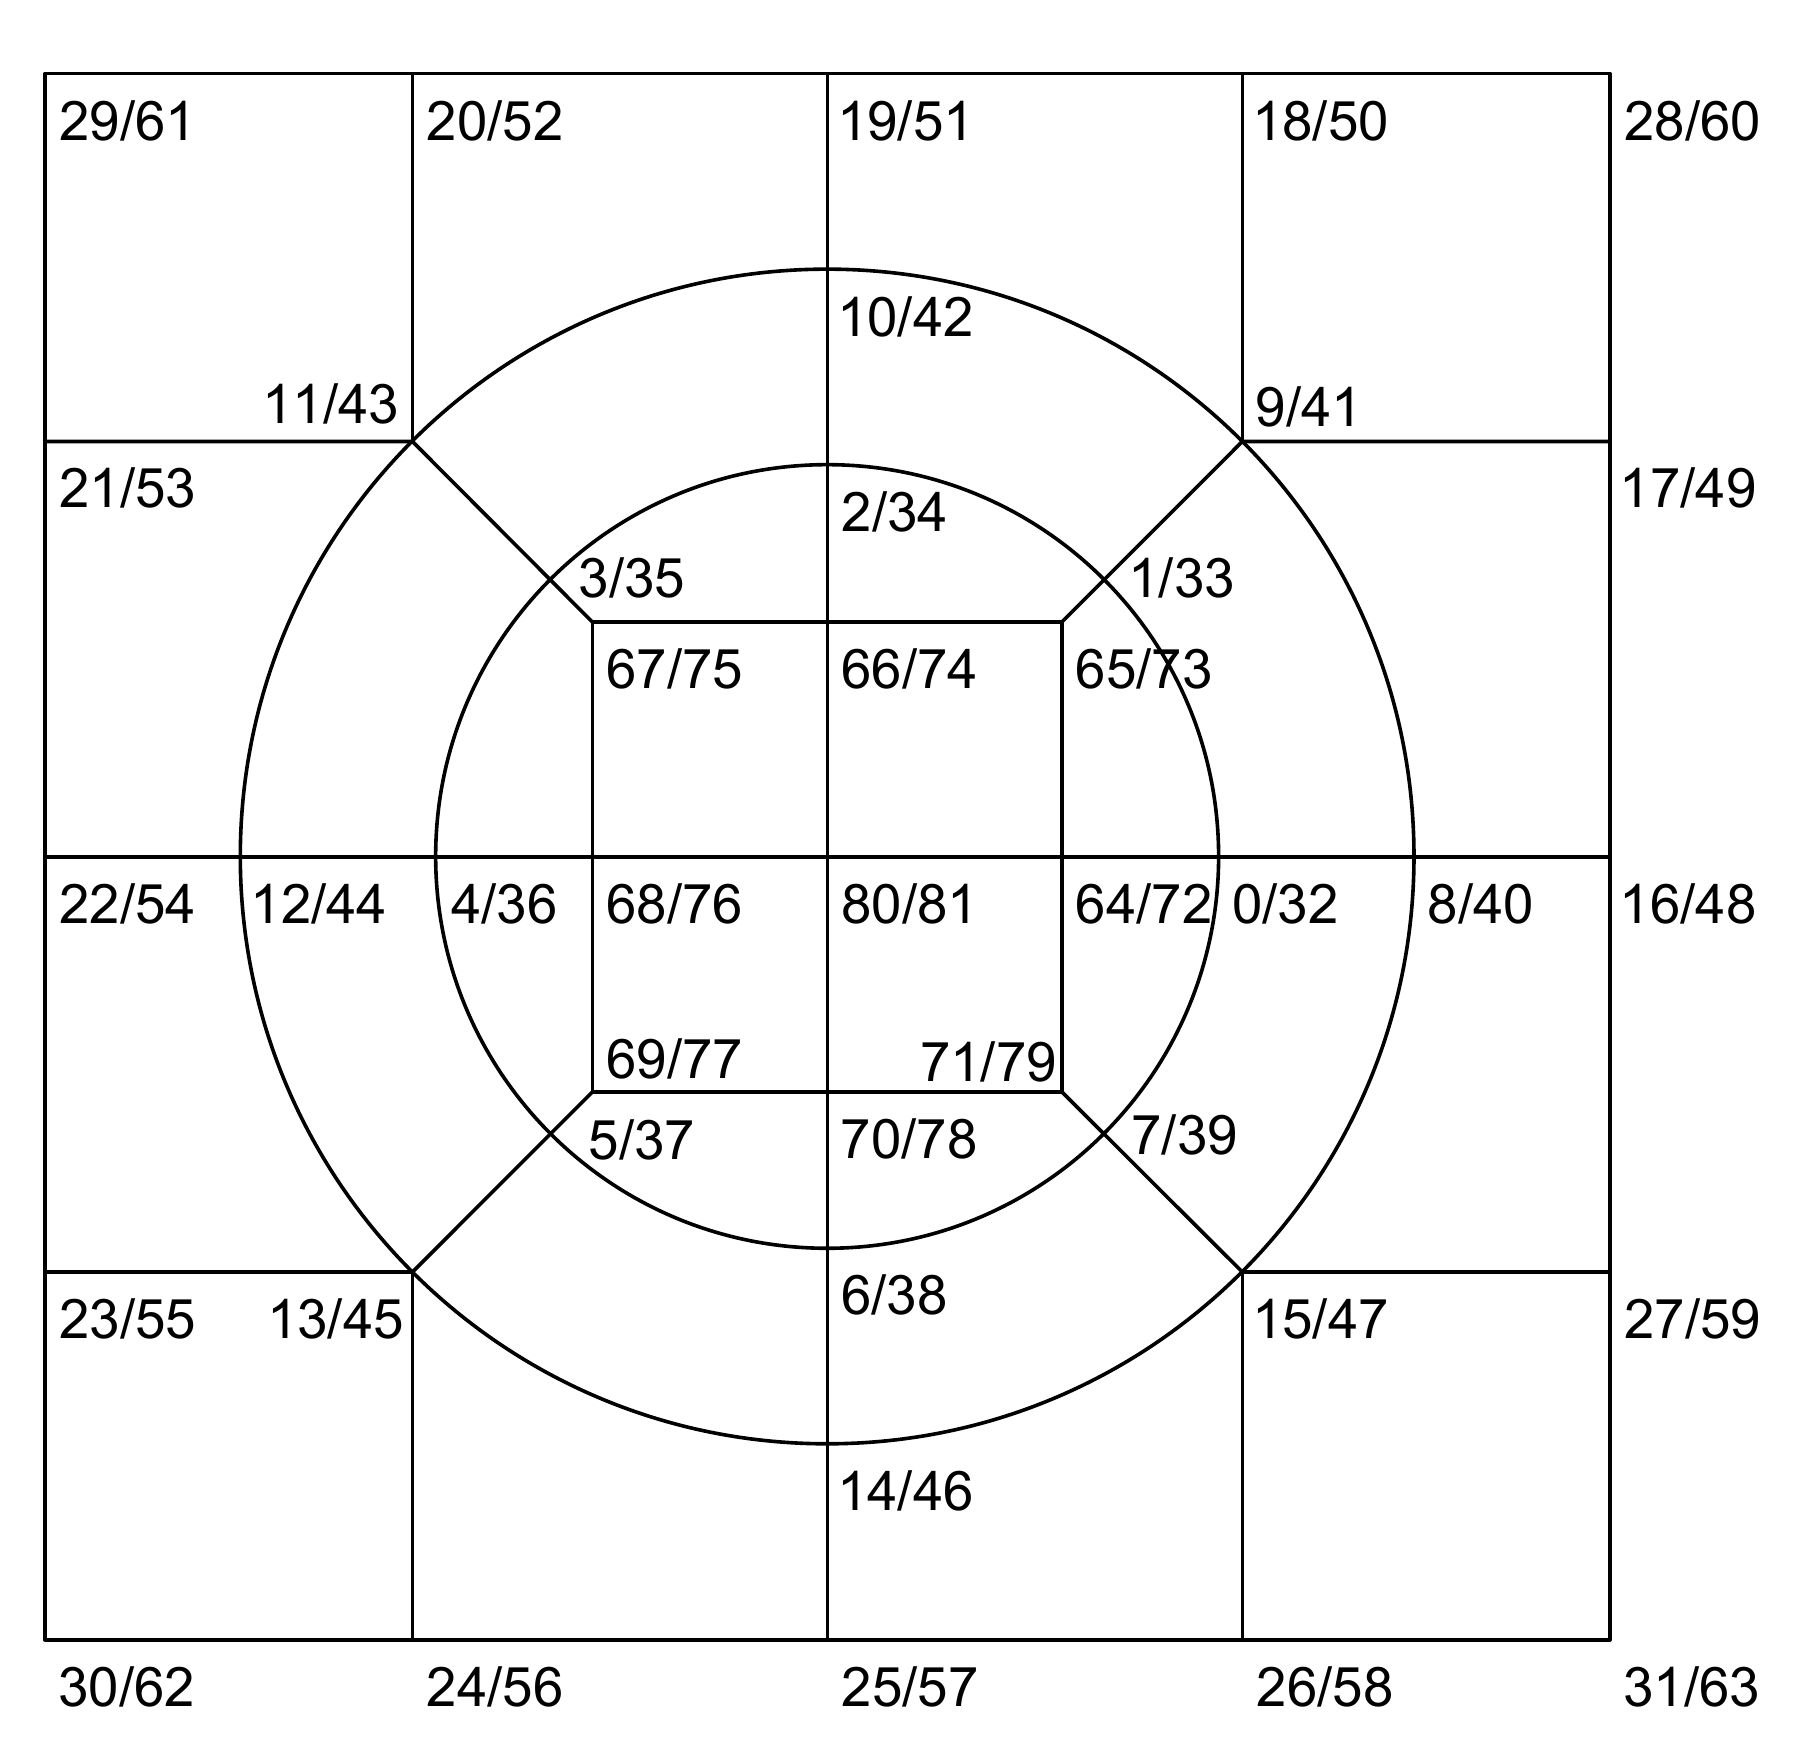
\includegraphics[width=3.75in]{Figures/2D-Labeled-Cube}
\par\end{centering}
\begin{centering}
(b)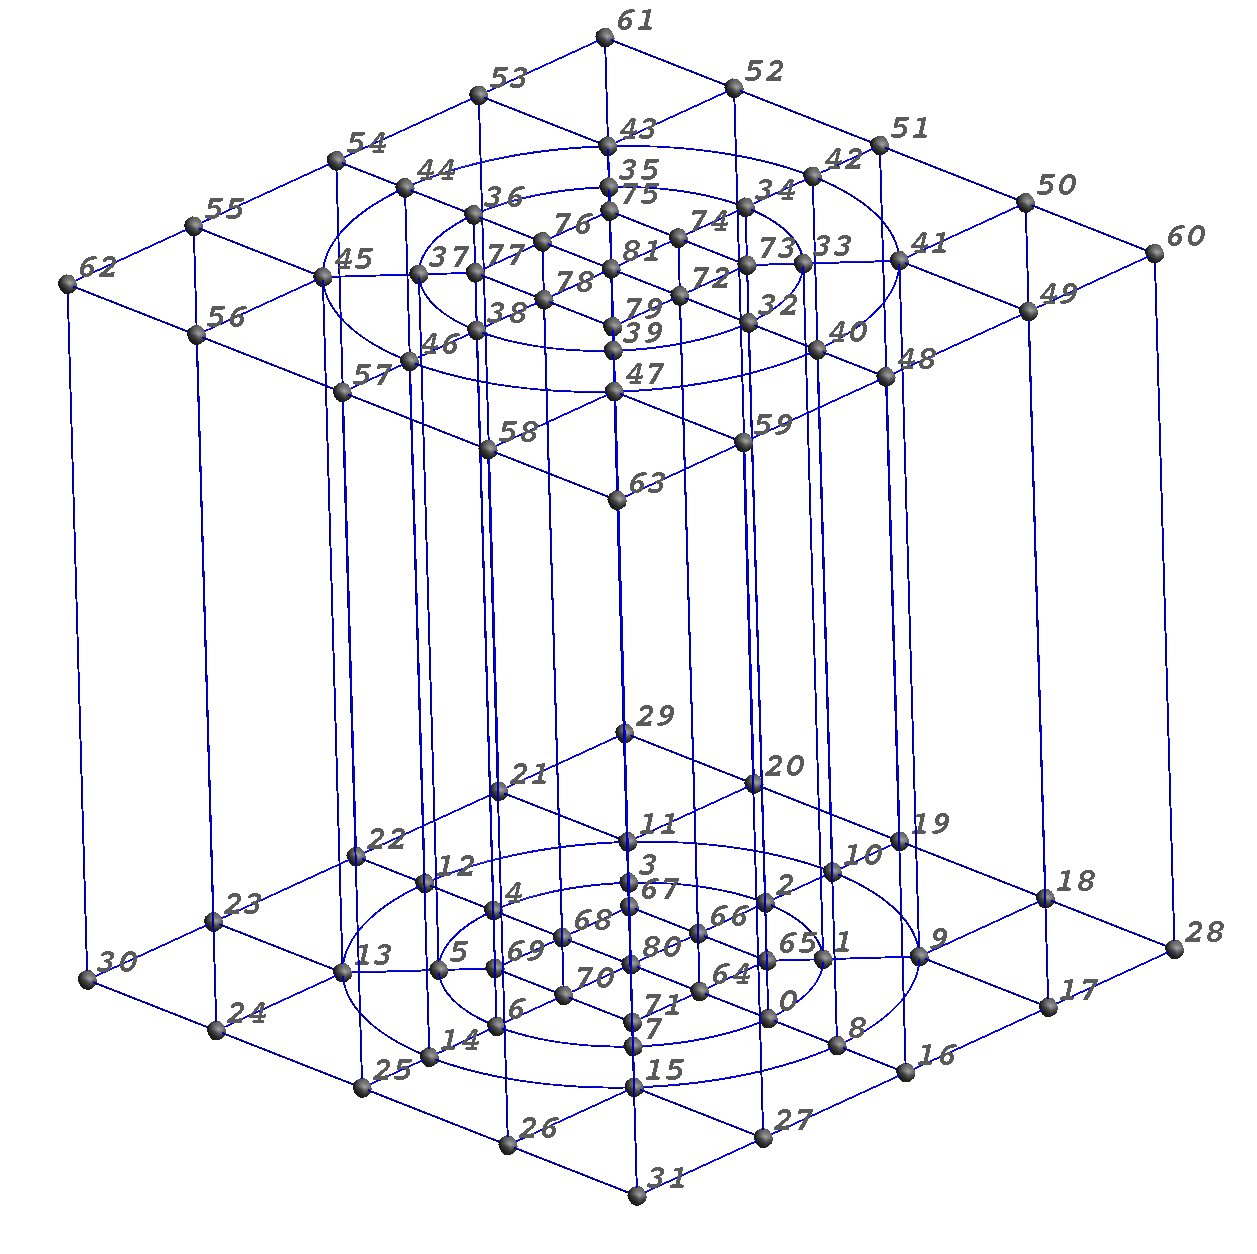
\includegraphics[width=3.75in]{Figures/3D-Labeled-Cube3-Size30Font4b}
\par\end{centering}
\caption{\label{fig:blockMesh}Vertex indices shown in (a) 2D and (b) 3D view
of a cylindrical stem in a rectangular box.}
\end{figure}

%\vfill

\newpage\null
\vfill
\begin{figure}[H]
\begin{centering}
(a)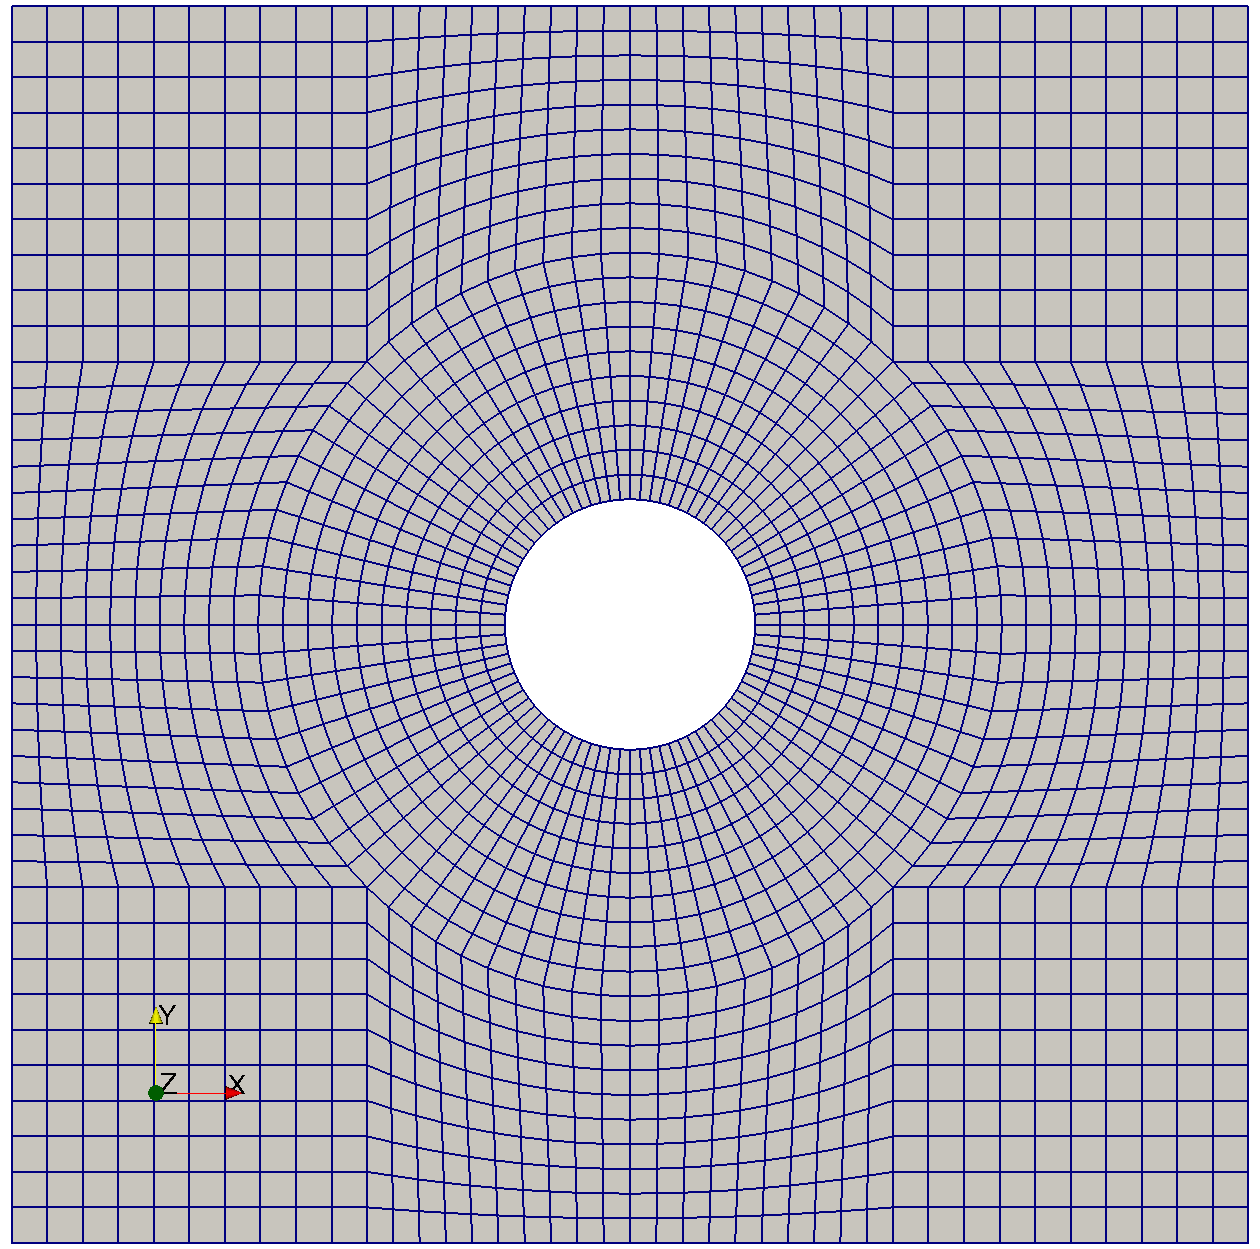
\includegraphics[width=3.75in]{Figures/mesh-empty-cylinder-in-z2-2019-10-13-20-51-19-PM}
\par\end{centering}
\begin{centering}
(b)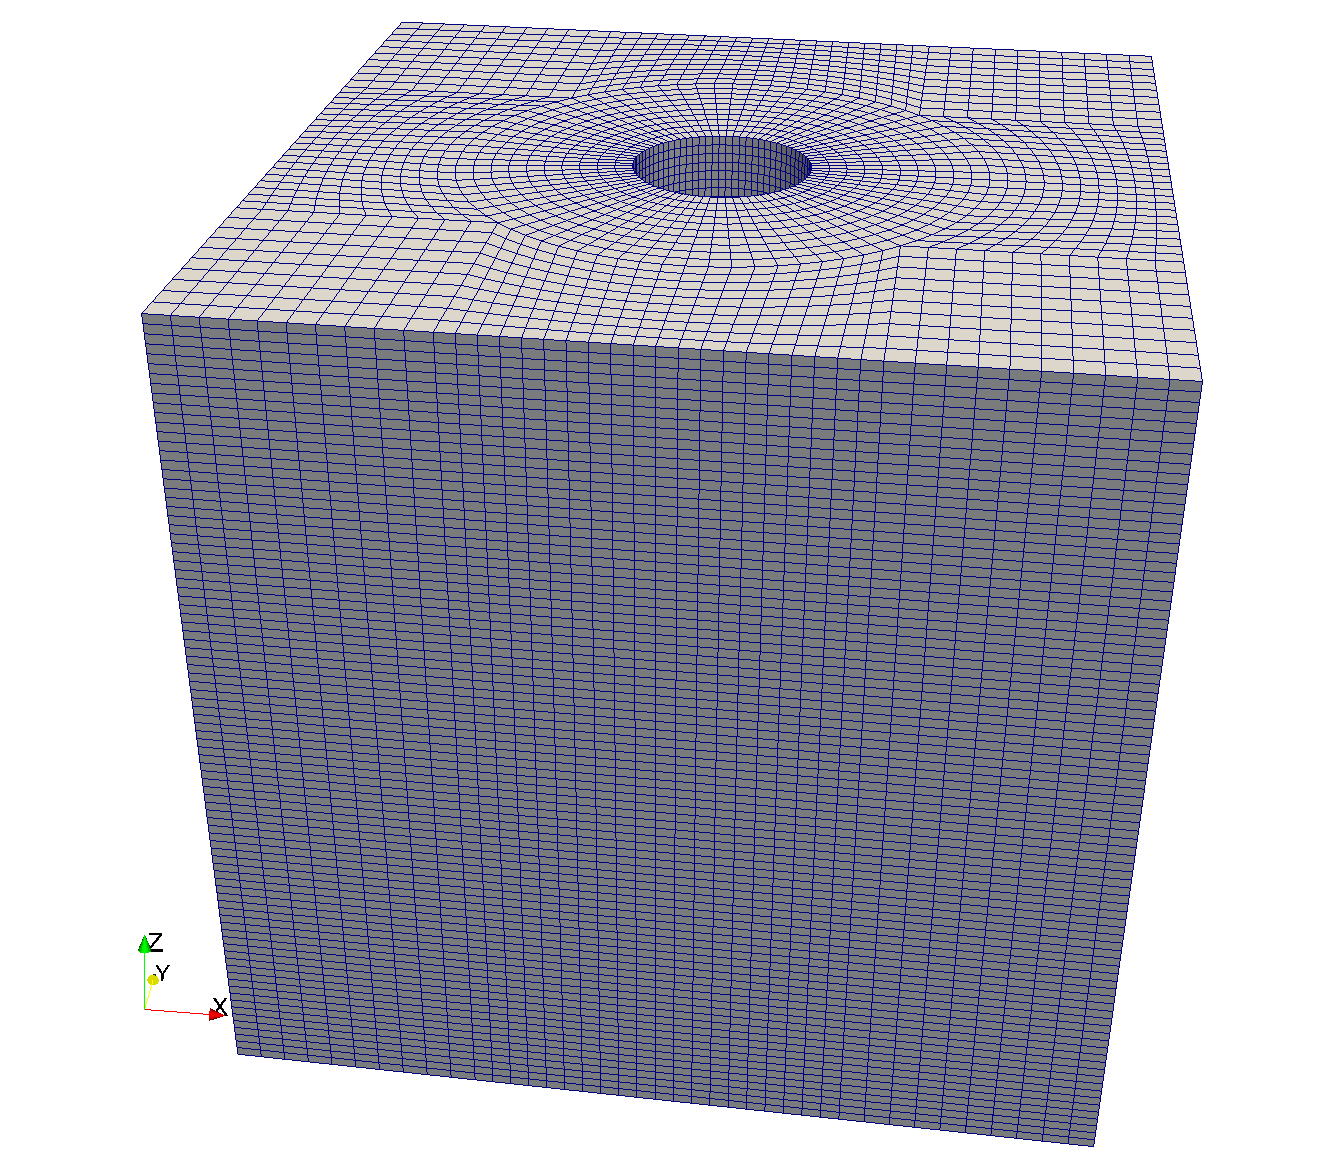
\includegraphics[width=3.75in]{Figures/mesh-empty-cylinder-3d2-2019-10-13-20-52-33-PM}
\par\end{centering}
\caption{\label{fig:emptyStem}Mesh grid structure outside a rigid cylindrical
stem, normally embedded on the bottom (bed) surface: (a) 2D top-view
and (b) 3D side-view.}
\end{figure}

\vfill$\phantom{.}$
